\documentclass{llncs}
\usepackage{amsmath,amssymb}
\usepackage{graphicx}

\title{Visibility in Discrete Geometry: an application to discrete geodesic}
\author{David Coeurjolly}


\newtheorem{defi}{Definition}
\newtheorem{prop}{Proposition}
\newtheorem{theo}{Theorem}

\begin{document}
\maketitle


\section{intro}

We use the arithmetical definition of discrete straight lines presented by Reveill\`es \cite{rev91},
such that $p(x,y)$ belongs to a discrete straight line $D(a,b,\mu,\omega)$  (with $a,b,\mu,\omega  \in
\mathbb{Z}$ and $a\wedge b=1$) if it satisfies : $\mu \leq ax-by < \mu+\omega$. A 8-connected discrete straight line,
also called {\it naive}, is obtained by considering a width $\omega$ equal to $\max(|a|,|b|)$.




In order to make a link between the discrete visibility  and the Euclidean one, we consider an
Euclidean domain $\mathcal{E}$ where boundaries and obstacle are defined by polylines such that vertices are
pixels in $\bar\mathcal{D}$ (see Figure \ref{fig:domaine}). Using this definition, obstacles can be
polygons, polylines or points. The visibility in $\mathcal{E}$ is defined as the classical Euclidean
visibility in computational geometry (see for example \cite{deberg}).

According to this definition, we have the followed property:

\begin{prop}
Let $s$ and $t$ pixels in $\mathcal{D}$, we have:
\begin{center}
\begin{tabular}{ccc}
$s$ and $t$ are visible in $\mathcal{E}$ & $\Leftrightarrow$ & $v(s,t)$
\end{tabular}
\end{center}
\end{prop}

\noindent{\it Proof:} If we have $v(s,t)$, all pixels in the discrete straight line belong to
$\mathcal{D}$ and the distance between each pixel in $\bar{\mathcal{D}}$ and the Euclidean segment
$[s,t]$ is strictly greater than 0. Thus, $s$ and $t$ are visible in $mathcal{E}$. To prove the
symmetric implication, we consider an Euclidean segment $[s,t]$ that belongs to $\mathcal{E}$.A
FINIR SI TOUT FOIS C'EST VRAI....




\begin{figure}[htbp]
  \begin{center}
    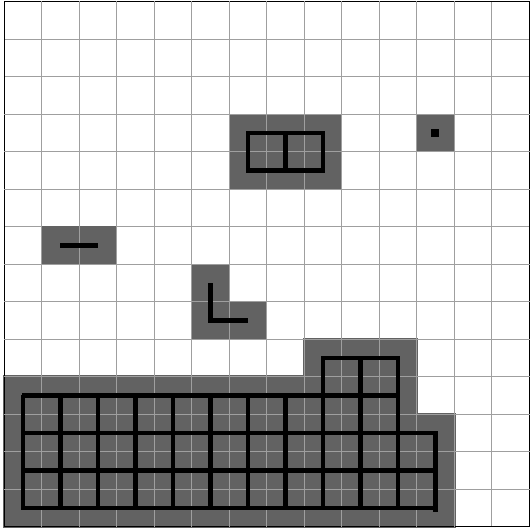
\includegraphics[width=4cm]{domaine2}
    \caption{tototo}
    \label{fig:domaine}
  \end{center}
\end{figure}


\subsection{Discrete straight line in non-convex domain}

We first recall some properties of discrete straight lines. We consider a naive straight line
$D(a,b,\mu)$ with $a<b$. The concerned pixels are solutions of $b$ diophantine  equations:
\begin{align*}
ax-by&=\mu\\
...& \\
ax-by&=\mu+b-1
\end{align*}

If we describe all possible discrete straight line between two point $s$ and $t$ such that $b/a$ is
the slope of such a segment ($a\wedge b=1$ and $a<b$), we obtain $2b-1$ diophantine equations:

\begin{align*}
ax-by&=-b+1\\
...&\\
ax-by&=b-1
\end{align*}

Let $\Delta(s,t)$ be the set of pixels solutions of these equations. Each $b$ consecutive equations form a naive straight line and there are $b-1$ such lines joining $s$
and $t$ (see Figure \ref{fig:droites}).

\begin{figure}[htbp]
  \begin{center}
    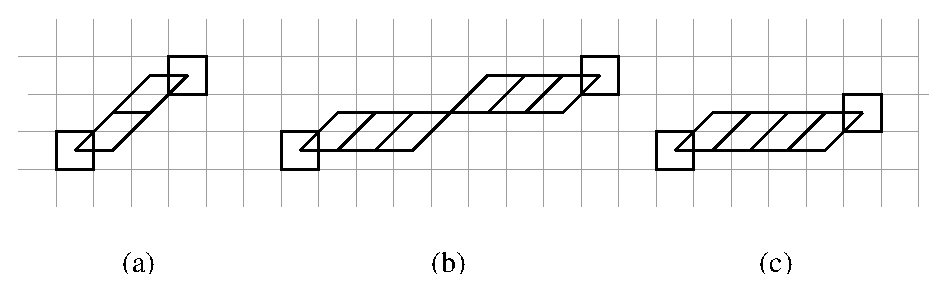
\includegraphics[width=8cm]{droites}
    \caption{Set of discrete naive lines joining two points : (a) the slope is $\frac{2}{3}$ so
      there are 3 possible naive lines, (b) the slope is $\frac{1}{4}$ so 4 possibles naive lines
      and (c) the slope is $\frac{1}{5}$ so 5 possible naive lines.}
    \label{fig:droites}
  \end{center}
\end{figure}


Based on these properties, we can present a sketch of the visibility algorithm: in order to decide
if we have $v(s,t)$, we compute all possible naive lines joining $s$ and $t$ and we remove naive
lines if one of its pixels belongs to $\bar{\mathcal{D}}$. If the resulting set of naive lines is
empty, $t$ is not visible from $s$. We define blocking pixels by:

\begin{defi}
Let $S$ denote pixels such that $S=\Delta(s,t)\cap\bar{\mathcal{D}}$, such points are called {\it blocking
  pixels} for the visibility between $s$ and $t$. Let $\mathcal{R}(s,t,S)$ denote the set of
resulting naive lines joining $s$ and $t$ and that do not contain pixels in $S$.
\end{defi}

And we have the important property that bound the number of points in $S$ that are interesting for
the visibility problem:

\begin{theo}
  The number of blocking pixels in $S$ that entirely define $\mathcal{R}$ is less or equal to 2.
\end{theo}


\noindent{\it Proof: } We consider two point $s$ and $t$ in $\mathcal{D}$ with slope $a/b$ ($a,b \in
\mathbb{Z}$ and $a\wedge b=1$). A discrete line solution is given by $b$ consecutive diophantine
equations in a  $2b-1$ possible set. Thus, let $M$ be a blocking point, we compute the diophantine
equation where $M$ belongs by computing the rest $r=ax-by$ \cite{debled}. Hence, we have to remove
this equation to the global set. Moreover, if ,for example, $r<0$, we must also remove all equations of rests $r'$
such that $r'<r$ because no $b$ consecutive equations can be found in $[-b+1,r]$ and so no
8-connected straight line can use these equations. Thus, all blocking points whose rests are lower
than $r$ do not affect the possible straight line $\mathcal{R}$. In general, since only one set on
$n$ consecutive equation with $b\leq n\leq 2b-1$ exits, this set is entirely defined by at most two blocking
points denoted $M_l$ and $M_r$ such that:
\begin{itemize}
\item $M_l$ have a rest $r_l$ such that $r_l<0$ and $r_l$ is the maximum rest of blocking points
  whose rest are less than 0 
\item $M_r$have a rest $r_r$ such that $r_r>0$ and $r_r$ is the minimum rest of blocking points
  whose rest are greater than 0
\end{itemize}

To illustrate this property, we consider $s=(0,0)$ and $t=(8,2)$,  we have $a=1$ and $b=4$. We
obtain the set of equations whose rests are:
\begin{displaymath}
-3,-2,-1,0,1,2,3
\end{displaymath}
We consider the blocking pixels $M_1=(1,1)$, $M_2=(2,1)$ and $M_3=(3,0)$ whose rests are $r_1=-3$,
$r_2=-2$ and $r_3=3$ (see Figure \ref{fig:exemple}). According to these points we have $M_l=M_2$ ($r_2>r_1$ and $r_1,r_2<0$) and
$M_r=M_3$ ($r_3>0$) and these two point entirely descirbe the possible set of discrete straight
line. In this example, $t$ is visible from $s$ because the number of resulting equations is greater
or equal to 4:
\begin{displaymath}
  \begin{array}[b]{c|}-3,-2,
  \end{array}\quad
  \overbrace{-1,0,1,2}^{D},\quad\begin{array}{|c}3
  \end{array}
\end{displaymath}

\begin{figure}[!ht]
  \begin{center}
    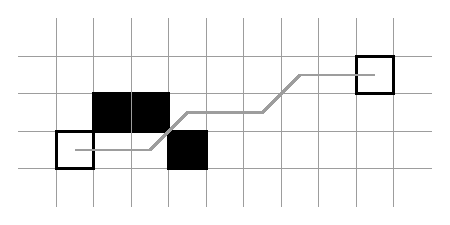
\includegraphics[width=5cm]{exemple}
    \caption{White pixels are $s$ and $t$ and black pixels are blocking pixels. The grey polyline
      represents the unique discrete straight line in $\mathcal{D}$ between $s$ and $t$.}
    \label{fig:exemple}
  \end{center}
\end{figure}


Based on these definitions, we have the property:
\begin{prop}
Let $s$ and $t$ in $\mathcal{D}$ and $M_l$ and $M_r$ in $\bar{\mathcal{D}}$ defined above, we have:
\begin{equation}
v(s,t) \Leftrightarrow r_r-r_l+1 \geq b
\end{equation}

Note that if there are neither such $M_l$ nor $M_r$, $r_l$ is set to $-b$ and $r_r$ to b.
\label{prop1}
\end{prop}

\subsection{Visibility Algorithm}

Based on prop. \ref{prop1}, we can design an algorithm to compute equivalences classes of the
visibility binary relation. We first detail the data structure associated to each pixel. At each
pixel, we associate  the structure:

\begin{center}
\begin{tabular}{|c|c|}
\hline
$x,y$ & position of $P$ in $\mathcal{D}$ relative to $s$\\
\hline$a,b$ & slope of the segment $[s,P]$ with $a\wedge b=1$\\
\hline$M_l$& extreme blocking pixel if it exists\\
\hline$M_r$ & extreme blocking pixel if it exists\\
\hline
\end{tabular}
\end{center}


We have two basis functions, the first one concern the visibility test according to
prop. \ref{prop1} and the second one concern the merging blocking point procedure.


\footnotesize
\vspace{0.5cm}
\hrule\hrule\vspace*{0.3cm}
\centerline{{\it Visibility(P)}}
\noindent \textsf{Input: point $P$\\
\noindent Output: {\tt True} if $P$ is visible from $s$ and {\tt False} if not\\
\\
\hspace*{0.5cm} Compute $r_l=aM_l.x-bM_l.y$ and $r_r=aM_r.x-bM_r.y$\\
\hspace*{1cm}{\it (if $M_l$ (resp. $M_l$) is not defined $r_l=-b$ (resp. $r_r=b$))}\\
\hspace*{0.5cm}{\bf Return} $(r_r-r_l+1 \geq b)$\\
}
\hrule
\normalsize

\footnotesize
\vspace{0.5cm}
\hrule
\hrule\vspace*{0.3cm}\centerline{{\it Merge\_Blocking\_Point(P,M)}}
\noindent \textsf{Input: point $P$ and a blocking point $M\in\bar{\mathcal{D}}$\\
\noindent Output: $P$ where extreme blocking point have been updated according to $M$
\\
\hspace*{0.5cm} Compute $r_l=aM_l.x-bM_l.y$ and $r_r=aM_r.x-bM_r.y$\\
\hspace*{1cm}{\it (if $M_l$ (resp. $M_l$) is not defined $r_l=-b$ (resp. $r_r=b$))}\\
\hspace*{0.5cm} Compute $r=aM.x-bM.y$\\
\hspace*{0.5cm} {\bf If} $(r<0)$ AND $(r>r_l)$ {\bf then}\\
\hspace*{1cm} $M_l\leftarrow M$\\
\hspace*{0.5cm}{\bf Else If} $r>0$ AND $(r<r_r)$ {\bf then}\\
\hspace*{1cm} $M_r\leftarrow M$\\
\hspace*{0.5cm}{\bf Return} $P$
}\\
\hrule
\normalsize

The visibility procedure starts from a point $s$ in $\mathcal{D}$ and then, using a classical
 breath-first tracking on the 8-adjacency graph,  propagates the visibility and blocking points to
 its neighbors. If a point in $\bar{\mathcal{D}}$ is met, we apply the merging function. This leads
 to s simple algorithm:


\footnotesize
\vspace{0.5cm}
\hrule\vspace*{0.3cm}
\centerline{{\it Visibility\_from\_one\_source(s,$\mathcal{D},\bar{\mathcal{D}}$)}}

\noindent \textsf{Input: source point $s$, the domain $\mathcal{D}$ and it complementary $\bar{\mathcal{D}}$\\
\noindent Output: Set of point in $\mathcal{D}$ visible from $s$\\
\noindent Temporary variables: a queue structure $Q$ to implement the breath-first tracking\\
\hspace*{0.5cm} Add $s$ to $Q$\\
\hspace*{0.5cm} {\bf While} $Q$ is not empty\\
\hspace*{1cm} remove first element of $Q$ denoted $l$ and mark $l$ as ``visible''\\
\hspace*{1cm} $B$ is the set of blocking points in $l$ neighborhood\\
\hspace*{1cm} {\bf For each} neighbors $n$ of $l$ not yet marked ``visible'' {\bf do}\\
\hspace*{1.5cm} propagate $l$'s blocking points to $n$\\
\hspace*{1.5cm} compute parameters $a,b$ of the segment $[s,n]$ (see below)\\
\hspace*{1.5cm} {\bf For each} blocking points in $B$ {\bf do}\\
\hspace*{2cm} Apply $Merge\_Blocking\_Point function$\\
\hspace*{1.5cm} {\bf IF} $Visibility(n)$ {\bf then}\\
\hspace*{2cm} append $n$ at the end of $Q$\\
\hspace*{0.5cm}{\bf EndWhile}
}\\
\hrule
\normalsize


\subsection{Complexity analysis}

The visibility test and the merging function is done in a constant time. A naive
implementation of $(a,b)$ calculus costs $O(log(n))$ where $n$ is the size of the data (Euclide
algorithm). However, a lot literature about discrete straight line recognition present an $O(1)$
cost if we propagate $(a,b)$ on a point $l$ to one of its neighbors
\cite{debled,dorst,bruckstein,mcillroy}. Finally, the global cost of the visibility algorithm in a
non-convex domain is linear in the number of pixel in $\mathcal{D}$ whatever the complexity of obstacle is.


\section{Discrete geodesics}

\subsection{avant}
metrique approchees -> dijkstra sur un graphe...
structure bucket
verwer, piper, cuisenaire


\subsection{metrique globale}

these Moreau..

on applique la visibilite pour une estimation des geodesiques.
Porbleme de l'approximation : pivot sur les pixels donc controle des sources 

toujours le probleme Danielson avec les voronoi : avec une propagation en 8-voisins on risque de
perdre dans le Dijkstra

solution : on memorise des visibilite multiples lorsqu'il y a mix et fusion. (borner l'erreur sur la
fusion de front pour que tout le monde se trouve dans le mm bucket et ensuite fusion des sources).




convergence mulitgrille avec convergence DSS ?


\section{Conclusion and future work}

3d, surface...





\begin{lem}
The binary relation defined by lemma 1 is symmetric
\end{lem}

\noindent{\it Proof}: we have to proof that $v(s,t) \Leftrightarrow v(t,s)$.

In fact, if we associate to each obstacle the domain $\mathcal{S}(s,o_i)\cap\mathcal{S}(o_i,t)$,
the binary relationship defined above is symmettric. Moreover, we can only consider the domain
$\mathcal{S}(s,o_i)$.

If $\mathcal{S}(s,t) - \bigcup_{i=1..n}\left(\mathcal{S}(s,o_i)\cap\mathcal{S}(o_i,t)\right )=\emptyset $


First of all, $\mathcal{S}(s,t)=\mathcal{S}(t,s)$ by definition. If $\neg v(s,t)$, we have:
\begin{displaymath}
  \mathcal{S}(s,t) \subseteq \bigcup_{i=1..n}\mathcal{S}(s,o_i)
\end{displaymath}
Which means that all digitization of all straight line in   $\mathcal{S}(s,t)$ contain at least one
obstacle. If we suppose $v(t,s)$, we have:
\begin{displaymath}
  \mathcal{S}(s,t) - \bigcup_{i=1..n}\mathcal{S}(o_i,t) \neq \emptyset
\end{displaymath}




We first present a necessary condition for an obstacle to be a blocking point. We denote $s_{inf}$
(resp. $s_{sup}$) the point $(x,y-1)$ (resp. $(x,y+1)$) whre $(x,y)$ is the coordinates of $s$. In
the same way, we define $t_{inf}$ and $t_{sup}$ associated to $t$ and $o_{inf}$, $o_{sup}$
associated to an obstacle $o$. The domain vertices in the parameter space of $\mathcal{S}(s,t)$ are
straight lines in the primal space with leaning points are the above characterisitc points (cf
figure \ref{appui}).

\begin{figure}[htbp]
  \begin{center}
    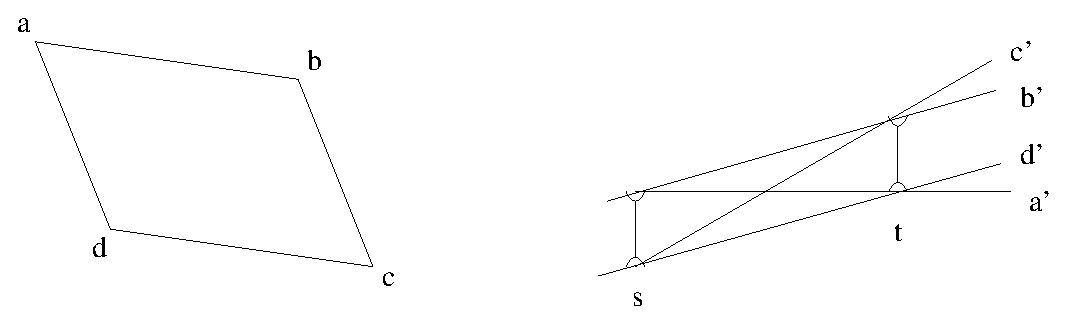
\includegraphics[width=8cm]{appui}
    \caption{A domain $\mathcal{S}(s,t)$ and the straight lines in the primal space associated to
      vertices of the domain.}
    \label{appui}
  \end{center}
\end{figure}

In order to restict the obstacle pixels $\mathcal{O}$ to blocking pixels  associated to $s$ and $t$,
we use the  following data structure: $\mathcal{C}_{inf}$  a double-linked list  of points $o_{inf}$
and $o_{sup}$   sorted  in  a  polar system  whom  $s_{inf}$  is  the   origin ,  in  the  same  way
$\mathcal{C}_{sup}$ is also a double-linked list of points $o_{inf}$ and $o_{sup}$ sorted in a polar
system whom $s_{sup}$ is the origin.

Given this structure, we have the porpery:

\begin{prop}
  An obstacle $o$ is a blocking pixel for the visibility problem $v(s,t)$ if and only if at least
  one extremity of $o$ ($o_{inf}$ or $o_{sup}$) verifies one of these predicats:
\begin{itemize}
  \item the extremity belongs to the angular sector $(s_{inf},t_{inf},t_{sup})$
  \item the extremity belongs to the angular sector $(s_{sup},t_{inf},t_{sup})$
  \item the extremity belongs to the strip defined by lines $(s_{sup},t_{sup})$ and $(s_{inf},t_{inf})$
\end{itemize}
\end{prop}









\end{document}